\documentclass[letterpaper]{article}
\title{CSE 550 Introduction to Systems Research \\ Problem Set 2}

\usepackage{balance}  % to better equalize the last page
\usepackage{graphicx}
\usepackage{times}    % comment if you want LaTeX's default font
\usepackage{url}      % llt: nicely formatted URLs
\usepackage{graphicx}
\usepackage{tabularx}
\usepackage{float}
\usepackage{color}
\usepackage{url}
\usepackage[noend]{algpseudocode}
\usepackage{algorithm}
\usepackage{verbatim}
\usepackage{mathtools}
\usepackage{caption}
\usepackage{subcaption}
%\usepackage{amsmath}
\let\proof\relax
\let\endproof\relax
\usepackage{amsthm}
\usepackage{thmtools}
\usepackage{xspace}
\usepackage{multirow}
\newcommand{\field}[1]{\mathbb{#1}} 
\newcommand{\hide}[1]{#1}
\newcommand{\pd}[2]{\frac{\partial #1}{\partial #2}}
\providecommand{\m}[1]{\mathbf{#1}}
\providecommand{\norm}[1]{\left\|#1\right\|}
\providecommand{\sign}[1]{\text{sign}\left(#1\right)}
\DeclareMathOperator*{\argmin}{arg\,min}
\providecommand{\what}{\m{\hat{w}}}

\begin{document}
\author{Marco Tulio Correia Ribeiro, Shrainik Jain\\ 1323300, 1323338}
\maketitle

\section{Implementation}
The base system is a set of Nodes, each running a PaxosHandler instance and a Broker which acts as a middleware to interpret client requests. All the communication is done using the Apache Thrift Framework. Any client can contact Broker at any node, with a command of the form {\em Lock mutexId clientId} or {\em Unlock mutexNo clientId}. The Broker relays the commands to the PaxosHandler in the same Node. \\

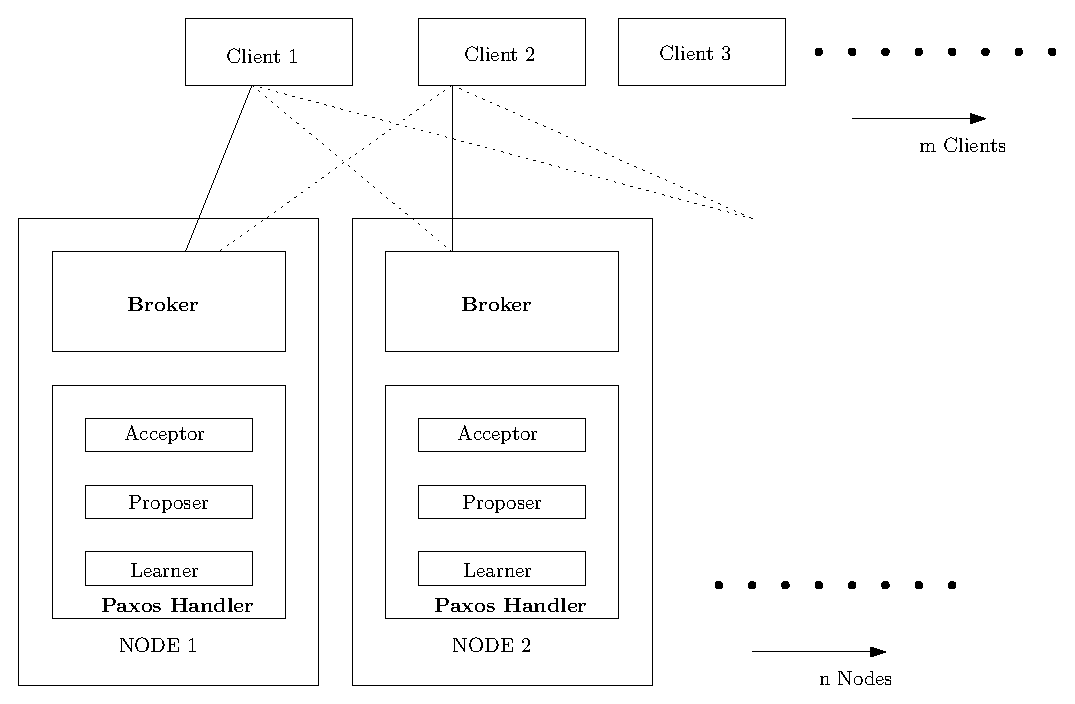
\includegraphics[width = 4.5in, keepaspectratio]{Architecture.eps}\\
\subsection{Normal operation}
PaxosHandler implements {\em leader Paxos}. Upon receiving a run command request, a node checks if it is the leader, if true, it starts an instance of Paxos with the value as the command recieved. If the node recieving the client request is not the leader, it asks the leader to run the command.\\
Each node has an id. At the start, the node with id 0 is set as the leader. In addition, each node also maintains the following state variables:
\begin{itemize}
\item current\_proposal\_number: This starts with 0 for all nodes. Its like a seed to calculate the actual proposal number for Paxos instances. Proposal number is calculated as \textbf{current\_proposal\_number * 1000 + my\_id}. Under normal operations, current\_proposal\_number is never changed.
\item An array of all the values accepted so far, indexed by instance number.
\item An array of the proposal number promised so far, indexed by instance number.
\end{itemize}

\subsection{Scenario where a node fails}
Node or communication failures are detected in the system when any node can't open a transport connection to some other node. In such a scenario \textbf{an exception is thrown, but its fine becuase we catch that exception and act accordingly}. Two possible situations could happen:
\begin{itemize}
\item Leader can't open a connection to some acceptor. 
\item A non leader can't open a connection to a leader while asking to start a new instance of Paxos.
\end{itemize}
The first situation is easily dealt with, the leader simply ignores the failure and contacts acceptor on some other node and keeps doing this till it gets a majority. The second situation means that some node can't communicate with the leader. This could either be becuase the leader is down or because the communication link is broken, in either case, the node which gets this exception, does a broadcast to all other nodes to elect a new leader whose id is old\_leader + 1. Elect new leader algorithm just udpates the id of leader on each node and also increases the value of current\_proposal\_number by 1. Further, if a node sees that its the new leader, it calls PrepareFuture on a majority of nodes. PrepareFuture updates the list of promised proposal number for all future instances to \textbf{current\_proposal\_number * 1000 + new\_leader\_id}. This ensures that if the older leader comes up in the future, it will always see a proposal number promised to be greater than what it proposes and thus understand that it is not the leader anymore. When this happens the older leader figures out who the new leader is (Figuring out the new leader is easy enough since we maintain a convention of proposal numbers to end with the leader id).

\section{Assumptions}
\begin{itemize}
\item For the sake of the assignment, we assume that the number of nodes is less than 1000.
\item Reconfiguration and recovery is not supported.
\item Client does the error handling itself. i.e. if the there is an error in the communication between client and a node, the client implements the retry/ignore logic.
\end{itemize}
\section{Running the code}
To ease the starting of the servers and brokers, we are submitting a few scripts.
\begin{itemize}
\item {\em start\_nodes.py}: Starts as many nodes (broker and paxos handlers) as given via argument. Usage:
\begin{verbatim}
start_nodes.py -l NUM_LOCKS -n NUM_NODES
\end{verbatim}
This will start a bunch of nodes as servers running on different ports on the localhost. And will also output the port numbers for the broker and paxoshandler on each node. After this you can just run the following commands on the client:
\begin{verbatim}
Broker-remote [-h host[:port]] Lock mutexNo ClientId
\end{verbatim}
Or
\begin{verbatim}
Broker-remote [-h host[:port]] Unlock mutexNo ClientId
\end{verbatim}

\item {\em test-failed-message.sh}: Script to simulate failed messages. (Automatically calls start\_nodes.py)\\
This script starts 3 nodes and runs a few client requests and then issues an elect new leader (similar to what a node would do in case of message failure). 
\item {\em test-kill-leader.sh}: Script to kill a leader and see if the Paxos nodes are still working.\\
This script starts 3 nodes and after running a few client requests, kills the leader, then tries to run a few other commands. 
\item {\em test-kill-2-leaders.sh}: Script to kill one leader after another to see if the Paxos nodes are still working.
\begin{itemize}
\item Starts 5 nodes.
\item Runs a few client requests.
\item Kills the leader.
\item Runs some more client requests.
\item Kills the second leader.
\item Runs some more client requests.
\end{itemize}
\item {\em test-kill-2-nodes.sh}: Script to kill non-leader nodes to see if the Paxos nodes are still working.
\begin{itemize}
\item Starts 5 nodes.
\item Runs a few client requests.
\item Kills a non-leader.
\item Runs some more client requests.
\item Kills another non-leader.
\item Runs some more client requests.
\end{itemize}

\item {\em test-gap.sh}
\begin{itemize}
\item Starts 5 nodes. 
\item 
\item 
\item 
\item 
\end{itemize}

\end{itemize}

\end{document}